\documentclass{article}
\usepackage[top=1in, bottom=1in, left=1in, right=1in]{geometry}
\usepackage{polski}
\usepackage[utf8]{inputenc}
\usepackage{graphicx}
\begin{document}
\title{\huge\bfseries Sprawdzanie prawa Malusa}
\date{}
\author{}
\maketitle
\section{Wstęp teoretyczny}
\subsection{Cewka}
\textbf{Przepływ prądu stałego przez cewkę}\\
Podczas przepływu prądu przez cewkę, indukuje się w cewce siła elektromotoryczna. Zakładając, że indukcyjność cewki nie zmienia się, co zachodzi dla większości obwodów elektrycznych, wzór  wygląda następująco:
$$\epsilon = -L \frac{di}{dt}$$
$\epsilon - $ siła elektromotoryczna, $L - $ indukcyjność cewki, $i - $ natężenie prądu płynącego przez cewkę, $t - $ czas\\
Dla prądu stałego odpowiednikiem indukcyjności jest stała cewki:
$$C = \frac{H}{I}$$
$H-$ natężenie pola magnetycznego, $I-$ natężenie prądu\\\\
\textbf{Rezystancja cewki} to przepływ prądu przemiennego przez cewkę.
W obwodach prądu zmiennego sinusoidalnego, w stanie ustalonym napięcie na cewce wyprzedza o 90$^\circ$ prąd płynący w cewce.\\
\textbf{Rolą rdzenia w cewce} jest wzmacnianie pola magnetycznego wytwarzanego podczas podczas przepływu prądu przez uzwojenie elektromagnesu. Rdzeń wykonany jest ze stali miękkiej i dlatego nie magnesuje się trwale.\\
\textbf{Indukcyjność cewki} to zdolność obwodu do wytwarzania strumienia pola magnetycznego $\phi$ powstającego w wyniku przepływu przez obwód prądu elektrycznego. Jednostką indukcyjności jest $1 henr[H]$. Indukcyjność opisuje się jako stosunek tego strumienia i prądu, który go wytworzył:
$$L = k\frac{\phi}{i}$$
\textbf{Impedancja} to wielkość charakteryzująca zależność między natężeniem prądu i napięciem w obwodach prądu zmiennego. Impedancja idealnej cewki jest równa iloczynowi jej reaktancji i jednostki urojonej.
\subsection{Kondensator}
\textbf{Przepływ prądu przemiennego przez kondensator}\\
Doprowadzenie napięcia do okładek kondensatora powoduje zgromadzenie się na nich ładunku elektrycznego. 
Dla prądu przemiennego przez kondensator płynie prąd określony wzorem:
$$U_c(t) = U_0\sin (\omega t)$$
$$I_c=C\frac{dU_c}{dt}=CU_o\omega \cos (\omega t)$$
\textbf{Pojemność kondensatora} to pojemność określająca zdolność kondensatora do gromadzenia ładunku $$C = \frac{Q}{U}$$
$U-$ napięcie\\
\textbf{Reaktancja pojemnościowa kondensatora} to wielkość wiążąca prąd i napięcie na kondensatorze. Reaktancja jest mniejsza, im większa jest pojemność kondensatora i częstotliwość prądu. Wyraża się ją wzorem:
$$X_C= \frac{-1}{\omega C}=\frac{-1}{2\pi fC}$$
$\omega -$ Pulsacja, $f -$ częstotliwość w hercach, $j-$ jednostka urojona.\\
\textbf{Szeregowe i równoległe połączenia kondensatorów}\\
Podobnie jak rezystory i cewki, także kondensatory można łączyć w celu uzyskania pożądanej pojemności.\\
W połączeniu szeregowym pojemność zastępcza dana jest wzorem:
$$\frac{1}{C_z}=\frac{1}{C_1}+\frac{1}{C_2}+...+\frac{1}{C_n}$$
W przypadku połączenia równoległego kondensatorów pojemność zastępcza wyraża się zależnością:
$$C_z = C_1 + C_2 + ...+C_n$$
Taka zależność wynika z faktu, że ładunek elektryczny równolegle połączonych kondensatorów jest sumą ładunków zgromadzonych na kondensatorach.
\section{Opracowanie wyników pomiarów}
Charakterystyki prądowo-napięciowe $I = f(U)$ dla:\\\\
Cewki z rdzeniem, z zasilaniem układu prądem stałym:
\begin{center}
    \begin{tabular}{|c|c|c|c|}
    \hline
$I,mA$ & $u(I), mA$ & $U,V$ & $u(U), V$ \\ \hline
$6,7$ & $0,13$ & $0,504$ & $0,0032$\\ \hline
$13,3$ & $0,17$ & $1$ & $0,0035$\\ \hline
$19,9$ & $0,20$ & $1,497$ & $0,0037$\\ \hline
$26,7$ & $0,23$ & $2,018$ & $0,0040$\\ \hline
$33$ & $0,27$ & $2,48$ & $0,0042$\\ \hline
$40,6$ & $0,30$ & $3,05$ & $0,0045$\\ \hline
$46,2$ & $0,33$ & $3,51$ & $0,0048$\\ \hline
$54,5$ & $0,37$ & $4,088$ & $0,0050$\\ \hline
    \end{tabular}
\end{center}
Niepewność obliczona została na podstawie wzoru podanego przez producenta przyrządu pomiarowego tj. dla napięcia
$$0,05\% * x + 3 * 0,003\ V $$
oraz dla natężenia
$$0,5\% * x + 1 * 0,1\ mA$$
gdzie $x$ to mierzona wartość.
\begin{figure}[ht]
\centering
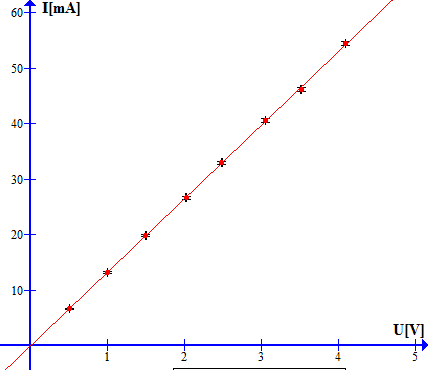
\includegraphics[height=8cm]{wykres_1.png}
\end{figure}\\
Przy pomocy funkcji w programie Excel 'REGLINP' wyznaczamy wzór lini trendu: $y = 13,2657x + 0,019$ oraz niepewność $u(a) = 0,1103$.\\
Odwrotność współczynnika 
$$R = \frac{1}{a}$$
prostej wyznacza rezystancję dla prądu stałego:
$$R = 0,0753823 \Omega$$ 
Aby obliczyć niepewność podanej wartości stosujemy wzór
$$u(R) = \sqrt[2]{(\frac{dR}{da}u(a))^2} = 0,0002063 \Omega$$
więc rezystancja jest równa
$$R = 0,0753823 \Omega \pm 0,2063 m \Omega$$
\\\\
Cewki z rdzeniem, z zasilaniem układu prądem przemiennym(zmieniając napięcie co 1V, zaczynając 0 kończąc na 8V):
\begin{center}
    \begin{tabular}{|c|c|c|c|}
    \hline
$I,mA$ & $u(I), mA$ & $U,V$ & $u(U), V$\\ \hline
$1$ & $0,31$ & $0,98$ & $0,015$\\ \hline
$2,2$ & $0,32$ & $1,99$ & $0,020$\\ \hline
$3,2$ & $0,33$ & $2,949$ & $0,025$\\ \hline
$4,3$ & $0,34$ & $3,968$ & $0,030$\\ \hline
$5,3$ & $0,35$ & $5,007$ & $0,035$\\ \hline
$6,3$ & $0,36$ & $6,022$ & $0,040$\\ \hline
$7,3$ & $0,37$ & $6,964$ & $0,045$\\ \hline
$8,3$ & $0,38$ & $7,973$ & $0,050$\\ \hline
    \end{tabular}
\end{center}
Niepewność obliczona została na podstawie wzoru tj. dla napięcia
$$0,5\% * x + 10 * 0,001\ V $$
oraz dla natężenia
$$1\% * x + 3 * 0,1\ mA$$
gdzie $x$ to mierzona wartość.
\begin{figure}[ht]
\centering
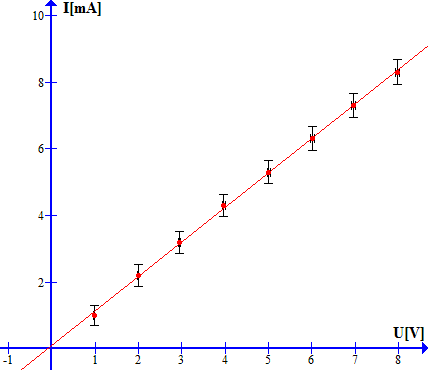
\includegraphics[height=8cm]{wykres_2.png}
\end{figure}\\
Przy pomocy funkcji w programie Excel 'REGLINP' wyznaczamy wzór lini trendu: $y = 1,0362x + 0,0938$ oraz niepewność $u(a) = 0,01351$.
Odwrotność współczynnika 
$$Z_L = \frac{1}{a}$$
prostej wyznacza impedancję $Z_L$ dla prądu zmiennego:
$$Z_L = 0,9650664 \Omega$$ 
Aby obliczyć niepewność podanej wartości stosujemy wzór
$$u(Z_L) = \sqrt[2]{(\frac{dZ_L}{da}u(a))^2} = 0,012583 \Omega$$
więc impedancja jest równa
$$Z_L = 0,9650664 \pm 12,583 m \Omega$$
Indukcyjność cewki wyliczamy ze wzoru
$$L = \frac{\sqrt{Z_L^2-R^2}}{2\pi f}$$
gdzie $R$ to obliczona wcześniej rezystancja, a $f$ to częstotliwość prądu przemiennego wynosząca $50 Hz$.
$$L = 3,063 H$$
Korzystając z propagacji niepewności obliczamy $u(L)$
$$u(L) = \sqrt{(\frac{Z_L}{2\pi f \sqrt{Z_L^2 - R^2}} \cdot u(Z_L))^2+(\frac{-R}{2\pi f \sqrt{Z_L^2-R^2}} \cdot u(R))^2} = 0,031 H$$
$$L = 3,063\ H \pm 0,029\ H$$\\\\
Cewki bez rdzenia, z zasilaniem układu prądem przemiennym:
\begin{center}
    \begin{tabular}{|c|c|c|c|}
    \hline
$I,mA$ & $u(I), mA$ & $U,V$ & $u(U), V$\\ \hline
$6,1$ & $0,36$ & $0,996$ & $0,015$\\ \hline
$12,5$ & $0,43$ & $2,027$ & $0,020$\\ \hline
$18,4$ & $0,48$ & $2,97$ & $0,025$\\ \hline
$24,6$ & $0,55$ & $3,982$ & $0,030$\\ \hline
$31$ & $0,61$ & $4,999$ & $0,035$\\ \hline
$37,5$ & $0,68$ & $6,042$ & $0,040$\\ \hline
$43,5$ & $0,73$ & $6,986$ & $0,045$\\ \hline
$51,4$ & $0,81$ & $8,02$ & $0,050$\\ \hline
    \end{tabular}
\end{center}
Niepewność obliczona została na podstawie wzoru tj. dla napięcia
$$0,5\% * x + 10 * 0,001\ V $$
oraz dla natężenia
$$1\% * x + 3 * 0,1\ mA$$
gdzie $x$ to mierzona wartość.
\begin{figure}[ht]
\centering
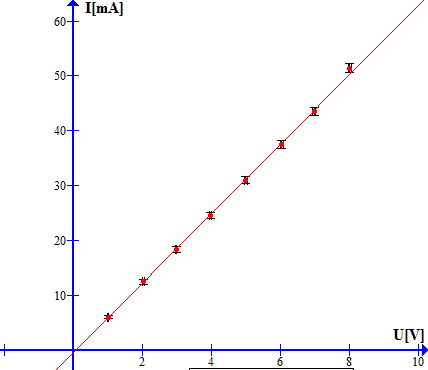
\includegraphics[height=8cm]{wykres_3.png}
\end{figure}\\
Przy pomocy funkcji w programie Excel 'REGLINP' wyznaczamy wzór lini trendu: $y = 6,3118x - 0,314$ oraz niepewność $u(a) = 0,0501$.\\
Odwrotność współczynnika 
$$Z_L = \frac{1}{a}$$
prostej wyznacza impedancję $Z_L$ dla cewki bez rdzenia dla prądu zmiennego:
$$Z_L = 0,1584 \Omega$$ 
Aby obliczyć niepewność podanej wartości stosujemy wzór
$$u(Z_L) = \sqrt[2]{(\frac{dZ_L}{da}u(a))^2} = 0,003546 \Omega$$
więc impedancja jest równa
$$Z_L = 0,1584 \Omega \pm 3,546 m \Omega$$
Indukcyjność cewki wyliczamy ze wzoru
$$L = \frac{\sqrt{Z_L^2-R^2}}{2\pi f}$$
gdzie $R$ to obliczona wcześniej rezystancja, a $f$ to częstotliwość prądu przemiennego wynosząca $50 Hz$.
$$L = 0,443447 H$$
Korzystając z propagacji niepewności obliczamy $u(L)$
$$u(L) = \sqrt{(\frac{Z_L}{2\pi f \sqrt{Z_L^2 - R^2}} \cdot u(Z_L))^2+(\frac{-R}{2\pi f \sqrt{Z_L^2-R^2}} \cdot u(R))^2} = 0,008 H$$
$$L = 0,443447\ H \pm 0,008\ H$$
\\\\
Kondensatora $C_1$, z zasilaniem układu prądem przemiennym:
\begin{center}
    \begin{tabular}{|c|c|c|c|}
    \hline
$I,mA$ & $u(I), mA$ & $U,V$ & $u(U), V$\\ \hline
$0,0123$ & $0,0031$ & $0,993$ & $0,015$\\ \hline
$0,25$ & $0,0055$ & $2$ & $0,02$\\ \hline
$0,371$ & $0,0067$ & $2,984$ & $0,025$\\ \hline
$0,497$ & $0,0080$ & $4,003$ & $0,030$\\ \hline
$0,624$ & $0,0092$ & $5,014$ & $0,035$\\ \hline
$0,746$ & $0,010$ & $5,978$ & $0,040$\\ \hline
$0,872$ & $0,012$ & $7$ & $0,045$\\ \hline
$0,998$ & $0,013$ & $7,974$ & $0,050$\\ \hline
    \end{tabular}
\end{center}
Niepewność obliczona została na podstawie wzoru tj. dla napięcia
$$0,5\% * x + 10 * 0,001\ V $$
oraz dla natężenia
$$1\% * x + 3 * 0,001\ mA$$
gdzie $x$ to mierzona wartość.
\begin{figure}[ht]
\centering
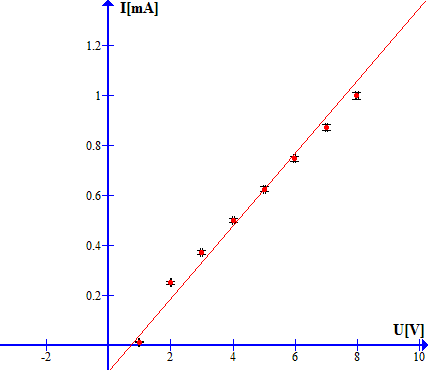
\includegraphics[height=8cm]{wykres_4.png}
\end{figure}\\
Przy pomocy funkcji w programie Excel 'REGLINP' wyznaczamy wzór lini trendu: $y = 0,1458x - 0,1069$ oraz niepewność $u(a) = 0,00021$.\\
Odwrotność współczynnika 
$$X_C = \frac{1}{a}$$
prostej wyznacza reaktancję pojemnościową $X_C$ kondensatora $C_1$:
$$X_C = 6,85871 \Omega$$ 
Aby obliczyć niepewność podanej wartości stosujemy wzór
$$u(X_C) = \sqrt[2]{(\frac{dX_C}{da}u(a))^2} = 0,013 \Omega$$
więc reaktancja pojemnościowa jest równa
$$X_C = 6,85871 \Omega \pm 13 m \Omega$$
Pojemność $C_1$ obliczamy ze wzoru
$$C_1 = \frac{1}{2\pi fX_C} = 464,096 \mu F$$
Korzystając z propagacji niepewności obliczamy $u(C)$
$$u(C) = \sqrt{(-\frac{1}{2\pi f X_C^2} \cdot u(X_C))^2} = 0,55 \mu F$$
$$C = 464,096 \mu F \pm 0,55 \mu F$$
\\\\
Kondensatora $C_2$, z zasilaniem układu prądem przemiennym:
\begin{center}
    \begin{tabular}{|c|c|c|c|}
    \hline
$I,mA$ & $u(I), mA$ & $U,V$ & $u(U), V$\\ \hline
$0,064$ & $0,0036$ & $1,023$ & $0,015$\\ \hline
$0,125$ & $0,0043$ & $2$ & $0,02$\\ \hline
$0,188$ & $0,0049$ & $3,005$ & $0,025$\\ \hline
$0,254$ & $0,0055$ & $4,035$ & $0,030$\\ \hline
$0,313$ & $0,0061$ & $5,009$ & $0,035$\\ \hline
$0,374$ & $0,0067$ & $5,992$ & $0,040$\\ \hline
$0,435$ & $0,0074$ & $7,03$ & $0,045$\\ \hline
$0,504$ & $0,0080$ & $8,045$ & $0,050$\\ \hline
    \end{tabular}
\end{center}
Niepewność obliczona została na podstawie wzoru tj. dla napięcia
$$0,5\% * x + 10 * 0,001\ V $$
oraz dla natężenia
$$1\% * x + 3 * 0,001\ mA$$
gdzie $x$ to mierzona wartość.
\begin{figure}[ht]
\centering
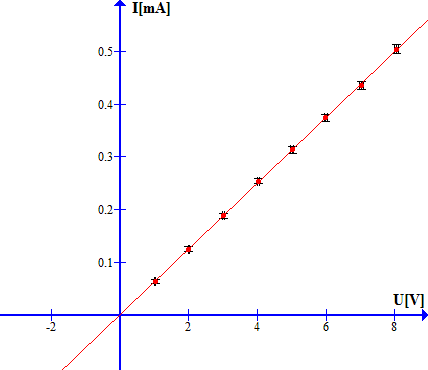
\includegraphics[height=8cm]{wykres_5.png}
\end{figure}\\
Przy pomocy funkcji w programie Excel 'REGLINP' wyznaczamy wzór lini trendu: $y = 0,0623x - 0,0005$ oraz niepewność $u(a) = 0,00013$.\\
Odwrotność współczynnika 
$$X_C = \frac{1}{a}$$
prostej wyznacza reaktancję pojemnościową $X_C$ kondensatora $C_2$:
$$X_C = 16,05136 \Omega$$ 
Aby obliczyć niepewność podanej wartości stosujemy wzór
$$u(X_C) = \sqrt[2]{(\frac{dX_C}{da}u(a))^2} = 0,03349 \Omega$$
więc reaktancja pojemnościowa jest równa
$$X_C = 16,05136 \Omega \pm 33,49 m \Omega$$
Pojemność $C_2$ obliczamy ze wzoru
$$C_2 = \frac{1}{2\pi fX_C} = 198,307 \mu F$$
Korzystając z propagacji niepewności obliczamy $u(C)$
$$u(C) = \sqrt{(-\frac{1}{2\pi f X_C^2} \cdot u(X_C))^2} = 0,30 \mu F$$
$$C = 198,307 \mu F \pm 0,30 \mu F$$
\\\\
Kondensatorów połączonych szeregowo, z zasilaniem układu prądem przemiennym:
\begin{center}
    \begin{tabular}{|c|c|c|c|}
    \hline
$I,mA$ & $u(I), mA$ & $U,V$ & $u(U), V$\\ \hline
$0,046$ & $0,0035$ & $1,039$ & $0,015$\\ \hline
$0,091$ & $0,0039$ & $1,998$ & $0,020$\\ \hline
$0,138$ & $0,0044$ & $3,015$ & $0,025$\\ \hline
$0,178$ & $0,0048$ & $3,972$ & $0,030$\\ \hline
$0,228$ & $0,0053$ & $4,998$ & $0,035$\\ \hline
$0,273$ & $0,0057$ & $6,005$ & $0,040$\\ \hline
$0,323$ & $0,0062$ & $7,054$ & $0,045$\\ \hline
$0,361$ & $0,0066$ & $7,909$ & $0,050$\\ \hline
    \end{tabular}
\end{center}
Niepewność obliczona została na podstawie wzoru tj. dla napięcia
$$0,5\% * x + 10 * 0,001\ V $$
oraz dla natężenia
$$1\% * x + 3 * 0,001\ mA$$
gdzie $x$ to mierzona wartość.
\begin{figure}[ht]
\centering
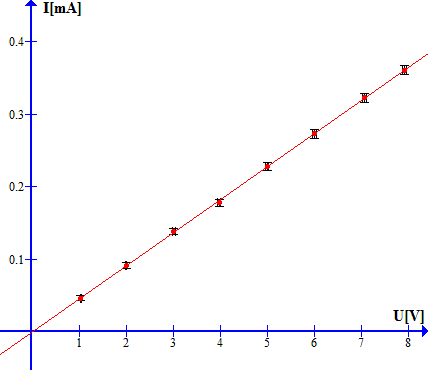
\includegraphics[height=8cm]{wykres_6.png}
\end{figure}\\
Przy pomocy funkcji w programie Excel 'REGLINP' wyznaczamy wzór lini trendu: $y = 0,0458x - 0,0013$ oraz niepewność $u(a) = 0,000062$.\\
Odwrotność współczynnika 
$$X_C = \frac{1}{a}$$
prostej wyznacza reaktancję pojemnościową $X_C$ szeregowo połączonych kondensatorów $C_1$ i $C_2$:
$$X_C = 21,83406 \Omega$$ 
Aby obliczyć niepewność podanej wartości stosujemy wzór
$$u(X_C) = \sqrt[2]{(\frac{dX_C}{da}u(a))^2} = 0,02955 \Omega$$
więc reaktancja pojemnościowa szeregowo połączonych kondensatorów $C_1$ i $C_2$ jest równa
$$X_C = 21,83406 \Omega \pm 0,02955 \Omega$$
Pojemność układu obliczamy ze wzoru
$$C = \frac{C_1C_2}{C_1+C_2} = \frac{464,096
 \cdot 198,307}{464,096 + 198,307} = 138,9388 \mu F$$
Korzystając z propagacji niepewności obliczamy $u(C)$
$$u(C) = \sqrt{(\frac{C_2(C_1+C_2)-(C_1C_2)}{(C_1+C_2)^2}u(C_1))^2 + (\frac{C_1(C_1+C_2)-(C_1C_2)}{(C_1+C_2)^2}u(C_2))^2} = 0,13 \mu F$$
$$C = 138,9388 \mu F \pm 0,13 \mu F$$
\\\\
\end{document}
